\documentclass[11pt,letterpaper]{article}
\PassOptionsToPackage{hyphens}{url}
\usepackage[margin=.83in,top=.8in,bottom=.8in,headheight=15pt]{geometry}
\usepackage[T1]{fontenc}
\usepackage{lmodern,amsmath,amssymb,mathtools,bm,booktabs,array,graphicx,tikz}
\usetikzlibrary{arrows.meta,positioning,calc,decorations.pathreplacing,patterns}
\definecolor{ink}{HTML}{17344D}\definecolor{accent}{HTML}{087E8B}\definecolor{pale}{HTML}{EDF5F5}\definecolor{gold}{HTML}{AD6B19}
\providecommand{\dd}{\,\mathrm{d}}\providecommand{\R}{\mathbb{R}}
\providecommand{\E}{\mathbb{E}}\providecommand{\Var}{\operatorname{Var}}
\providecommand{\Cov}{\operatorname{Cov}}\providecommand{\diag}{\operatorname{diag}}
\providecommand{\norm}[1]{\left\lVert#1\right\rVert}
\providecommand{\abs}[1]{\left|#1\right|}
\usepackage{microtype,hyperref,fancyhdr,enumitem,amsthm,sectsty,needspace}
\allsectionsfont{\raggedright}
\hypersetup{colorlinks=true,linkcolor=ink,urlcolor=accent,pdfauthor={Zan Ahmad},pdftitle={The circulation / Lecture notes}}
\setlength{\parindent}{0pt}\setlength{\parskip}{6pt}\linespread{1.07}
\setlist{itemsep=3pt,topsep=4pt,leftmargin=*}
\emergencystretch=2em\clubpenalty=10000\widowpenalty=10000
\pagestyle{fancy}\fancyhf{}\fancyhead[L]{\small Mathematical Cardiology}\fancyhead[R]{\small Lecture 1}
\fancyfoot[L]{\footnotesize Zan Ahmad}\fancyfoot[R]{\footnotesize\thepage}\renewcommand{\headrulewidth}{.3pt}
\newtheorem{proposition}{Proposition}\newtheorem{theorem}{Theorem}\newtheorem{lemma}{Lemma}
\theoremstyle{definition}\newtheorem{definition}{Definition}\newtheorem{example}{Example}
\numberwithin{equation}{section}
\begin{document}
{\small\scshape Mathematical Cardiology\hfill Lecture 1}\par\medskip
{\raggedright\hyphenpenalty=10000\exhyphenpenalty=10000\LARGE\bfseries\color{ink} The circulation\par}\medskip
{\small Lecture notes}\par\bigskip
The circulation is a closed transport system driven by a pump. To describe it mathematically, we first need to distinguish three things: where blood can go, how much passes a location, and what determines that amount. A route diagram answers the first question. A balance of volumes answers the second. A pressure--flow relation supplies an additional physical assumption. We shall keep these three ingredients separate and then put them together.

No calculus is needed for the initial construction. We begin with amounts transferred during a stated interval. The notation introduced here will remain useful when the rates later vary with time.

\section{The route and the direction convention}
\hypertarget{note-the-route-and-the-direction-convention}{}\label{note:the-route-and-the-direction-convention}
{\small \href{slides.html\#frame=the-circulation-as-a-closed-route\&step=1}{Slides for this section}}\par
Start at the left ventricle and follow one complete circuit:
\[
\begin{gathered}
\text{left ventricle}\longrightarrow\text{systemic vessels}\longrightarrow\text{right heart},\\
\text{right heart}\longrightarrow\text{pulmonary vessels}\longrightarrow\text{left heart}.
\end{gathered}
\]
The systemic vessels supply the tissues of the body; the pulmonary vessels carry blood through the lungs. These are two portions of one route, connected in series. Within each vascular bed, the many individual vessels branch and rejoin. Thus a diagram with one box for a bed describes its connections without specifying its internal geometry.

The four chambers and their valves refine this description. Systemic venous return enters the right atrium, crosses the tricuspid valve, and enters the right ventricle. The pulmonary valve leads to the pulmonary arteries. Pulmonary veins return to the left atrium; the mitral valve leads to the left ventricle, and the aortic valve leads to the systemic arteries. Arteries carry blood away from the heart and veins carry it toward the heart. Oxygen content does not define these names: the pulmonary arteries and veins illustrate why the distinction matters. Blood is red at both oxygen levels.

An arrow fixes a positive direction. It does not by itself prove that the flow has that sign. A passive connection can carry signed flow; a one-way valve needs a further constitutive rule. The diagram used here describes the principal adult route, omitting fetal connections, shunts and a separate coronary branch.
\begin{center}\begin{minipage}{.98\linewidth}\centering
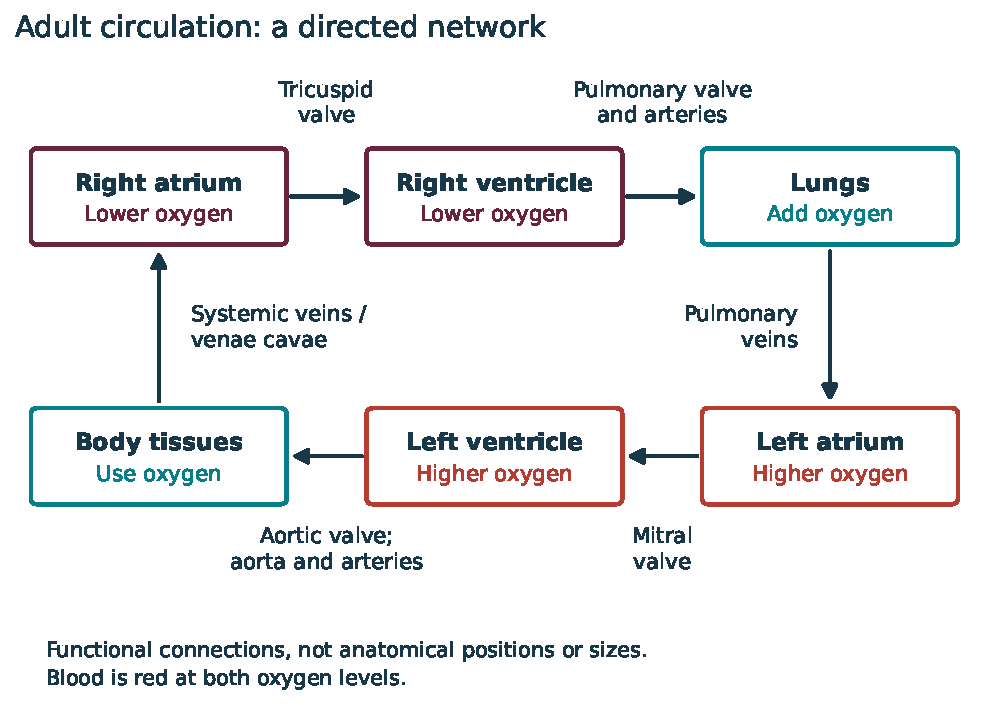
\includegraphics[width=.96\linewidth,height=.57\textheight,keepaspectratio]{network.pdf}\par\smallskip
{\small An original map of the principal adult route, including four chambers and the named valves. Arrows specify direction; boxes group structures. This is a connectivity diagram, not anatomical placement or a pressure calculation. Oxygen labels are categories; blood is red at both oxygen levels.}
\end{minipage}\end{center}
\section{An amount and a rate are different variables}
\hypertarget{note-an-amount-and-a-rate-are-different-variables}{}\label{note:an-amount-and-a-rate-are-different-variables}
{\small \href{slides.html\#frame=choose-the-quantity\&step=1}{Slides for this section}}\par
Write $V$ for a volume, in liters, and $Q$ for a volume flow rate, in liters per minute. If a constant flow crosses a selected section during an interval of length $\Delta t$, the volume passing that section is
\begin{equation}
\Delta V_{\rm passed}=Q\Delta t.
\end{equation}
The units explain the multiplication: $(\mathrm{L/min})(\mathrm{min})=\mathrm{L}$. For $Q=5\ \mathrm{L/min}$ and an interval of $30$ seconds,
\[
\Delta t=\frac{30}{60}\ \mathrm{min}=\frac12\ \mathrm{min},
\qquad \Delta V_{\rm passed}=5\cdot\frac12=2.5\ \mathrm{L}.
\]
This is volume passing a location, not volume accumulating inside a vessel. The same blood can cross that location again on a later circuit. Equating passing volume with newly created blood would confuse a transport measurement with a storage measurement.

A related multiplication gives average cardiac output. If the stroke volume is $V_s$ liters per beat and the heart rate is $F$ beats per minute, then $Q=FV_s$ when $V_s$ denotes the corresponding average per beat. The cancellation of beats leaves liters per minute. Increasing $F$ does not determine the change in $Q$ unless we also know how $V_s$ changes.
\section{Pressure enters through a difference}
\hypertarget{note-pressure-enters-through-a-difference}{}\label{note:pressure-enters-through-a-difference}
{\small \href{slides.html\#frame=the-pressure-drop\&step=1}{Slides for this section}}\par
Pressure is force divided by area. We use the customary cardiovascular unit mmHg, with both endpoint pressures referred to the same reference. For a connection oriented from an inlet to an outlet, define
\begin{equation}
\Delta P=P_{\rm in}-P_{\rm out}.
\end{equation}
Knowing $P_{\rm in}$ alone does not determine this difference. An inlet pressure of $95$ mmHg gives a drop of $90$ mmHg if the outlet is at $5$ mmHg, but only $45$ mmHg if the outlet is at $50$ mmHg.

Suppose we change only the numerical reference by adding a common constant $P_0$. Then
\[
(P_{\rm in}+P_0)-(P_{\rm out}+P_0)
=P_{\rm in}-P_{\rm out}.
\]
The common offset cancels. This is a statement about the same two pressures expressed relative to a different reference. It is not a statement that physically compressing a flexible vessel leaves its geometry unchanged. Pressure relative to the surrounding tissue will enter the storage law in the next lesson.
\section{A resistance is a physical assumption}
\hypertarget{note-a-resistance-is-a-physical-assumption}{}\label{note:a-resistance-is-a-physical-assumption}
{\small \href{slides.html\#frame=the-linear-resistance-law\&step=1}{Slides for this section}}\par
Consider a passive element with prescribed endpoint pressures, fixed effective geometry, and no storage or acceleration in the element. The simplest linear law is
\begin{equation}
\Delta P=RQ,\qquad Q=\frac{P_{\rm in}-P_{\rm out}}{R},\qquad R>0.
\end{equation}
Here $R$ has units $\mathrm{mmHg\,min/L}$. The positivity of $R$ makes flow follow the pressure drop. If the drop reverses, the signed flow reverses. This equation alone does not describe an ideal valve, nor does it describe the pressure increase across a working pump.

With $P_{\rm in}=95$ mmHg, $P_{\rm out}=5$ mmHg and $R=18\ \mathrm{mmHg\,min/L}$, the result is $Q=90/18=5\ \mathrm{L/min}$. At the same pressures, replacing $R$ by $36$ gives $Q=2.5\ \mathrm{L/min}$. More generally,
\[
\frac{Q_{\rm new}}{Q_{\rm old}}
=\frac{\Delta P_{\rm new}}{\Delta P_{\rm old}}
 \frac{R_{\rm old}}{R_{\rm new}},
\]
provided the old pressure difference and flow are nonzero. The familiar inverse relationship with resistance follows only after setting the pressure-difference ratio to one.

The graph of $Q$ against $\Delta P$ is a line through the origin with slope $1/R$. Equal pressures give zero flow, and doubling the pressure difference doubles the flow for the same resistance. These are mathematical checks of the stated law. They are not evidence that the effective resistance of a real vessel remains constant under every perturbation.
\begin{center}\begin{minipage}{.98\linewidth}\centering
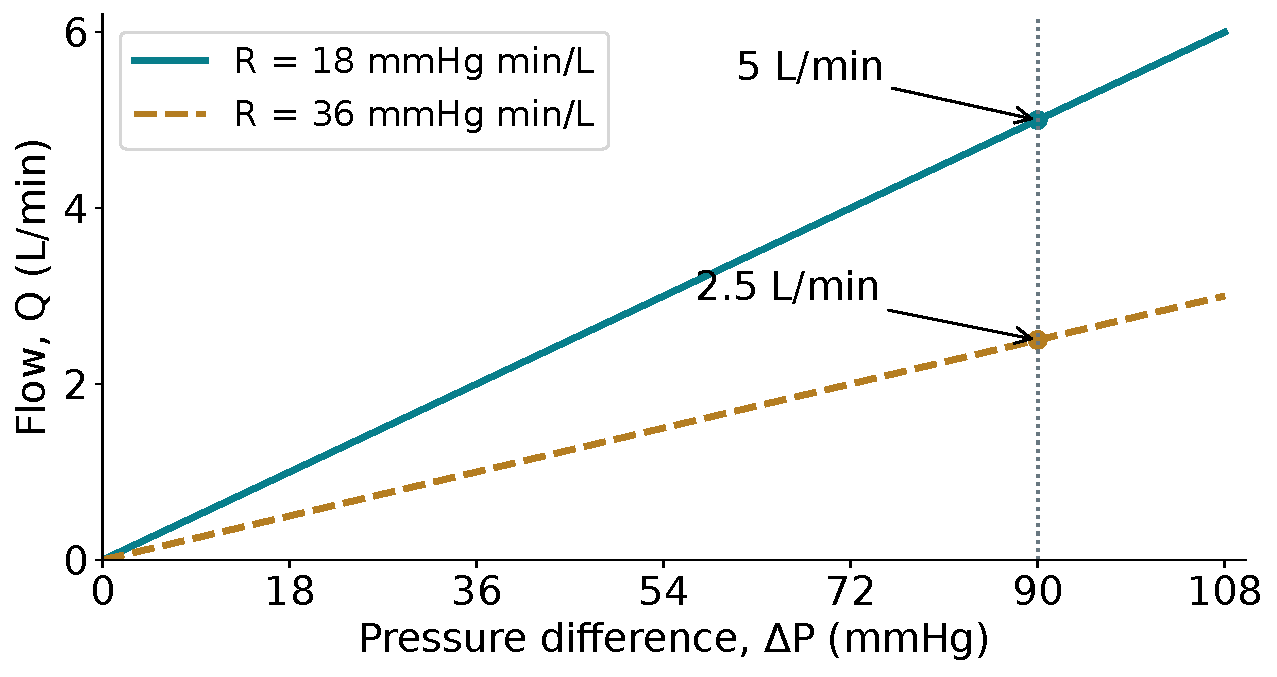
\includegraphics[width=.96\linewidth,height=.57\textheight,keepaspectratio]{presentation-figures/pressure-flow.pdf}\par\smallskip
{\small Original synthetic algebraic curves Q =\allowbreak{} $\Delta$P/R for R =\allowbreak{} 18 and 36 mmHg min/L. At $\Delta$P =\allowbreak{} 90 mmHg the marked flows are 5 and 2.5 L/min. Only resistance changes between the two marked comparisons; these are not measurements or whole-circulation predictions.}
\end{minipage}\end{center}
\section{Conservation begins with a chosen boundary}
\hypertarget{note-conservation-begins-with-a-chosen-boundary}{}\label{note:conservation-begins-with-a-chosen-boundary}
{\small \href{slides.html\#frame=count-volume-crossing-a-boundary\&step=1}{Slides for this section}}\par
Draw a boundary around a region. During an interval, every entering volume adds to its contents and every leaving volume subtracts from them. If rates are constant over that interval,
\begin{equation}
V_{\rm end}-V_{\rm start}
=\Delta t\left(\sum Q_{\rm in}-\sum Q_{\rm out}\right).
\end{equation}
The summation sign means that all connections crossing the boundary must be included. At a branch with one incoming flow and two outgoing flows, no accumulation means $Q_0=Q_1+Q_2$, not $Q_0=Q_1=Q_2$.

For two neighboring regions, let $q$ be their shared transfer, positive from region 1 to region 2. Their changes contain $-q\Delta t$ and $+q\Delta t$. Adding the two balances cancels this internal transfer. Repeating the cancellation over the entire closed circulation gives
\[
\Delta V_{\rm total}=0
\]
when no blood crosses the outer boundary. Conservation is therefore a property of the accounting, independent of our choice of resistance values.

A chamber can have different instantaneous inflow and outflow while satisfying this law: its volume changes. In a repeating state, volume returns to its starting value after a cycle. The volumes entering and leaving over that cycle must then be equal. This is why sustained average systemic and pulmonary flows agree in the simplified adult circuit without shunts. Equality of instantaneous flows is not required.
\section{Pressure rise supplied by the pump}
\hypertarget{note-pressure-rise-supplied-by-the-pump}{}\label{note:pressure-rise-supplied-by-the-pump}
{\small \href{slides.html\#frame=why-the-loop-needs-a-pump\&step=1}{Slides for this section}}\par
A loop made entirely of passive resistances cannot sustain a nonzero steady circulating flow without a pressure source. Going once around a closed route returns to the starting pressure, so the sum of all pressure changes is zero. If every passive element carries a common positive flow $Q$, its pressure drop is $R_iQ$. A pump must therefore supply a pressure rise equal to
\[
\Delta P_{\rm pump}=Q(R_1+\cdots+R_m).
\]
Without that rise, positivity of the resistances forces $Q=0$ in this simple steady series model. The heart supplies mechanical energy; it does not merely select a direction on the network.

Our single-resistance demonstration prescribes the endpoint pressures and calculates the division. It does not determine the pump law or the pressures elsewhere in the circulation. A useful comparison states which pressures are fixed, which resistance changes, and which flow is calculated. A useful extension then asks how the answer changes when those fixed pressures become unknowns coupled to a pump and elastic storage. That is the mathematical distinction between solving one element and solving the circulation.
\bigskip
\section*{Exercises}
\par\noindent\begin{minipage}{\linewidth}
\subsection*{MC01-E1. Read the network}
Use the original adult-network figure. This is a formative reasoning task; no coding is needed. Total: 10 points for feedback.

\textbf{a} Trace the route from the lungs through the left heart to body tissues. Name the two chambers and the two valves encountered in that part of the route.

\end{minipage}\par\medskip
\textbf{b} A classmate says every vein must carry oxygen-poor blood. Give a counterexample and explain the naming rule.

\textbf{c} Identify two features that this network preserves and two features it cannot tell you.

\par\noindent\begin{minipage}{\linewidth}
\subsection*{MC01-E2. Pressure differences and resistance}
Use the same passive linear-resistance assumption as the lesson. Values are synthetic. Total: 10 points for feedback.

\textbf{a} An inlet is at 84 mmHg, an outlet at 12 mmHg, and R =\allowbreak{} 24 mmHg min/L. Calculate $\Delta$P and Q, showing units.

\end{minipage}\par\medskip
\textbf{b} Both reported pressures are increased by 10 mmHg while R remains fixed. Does Q change? Explain using the new numbers.

\textbf{c} Route A has pressures 90 and 30 mmHg; route B has pressures 102 and 6 mmHg. Both have R =\allowbreak{} 24 mmHg min/L. Compute the flows and explain why comparing inlet pressures alone would be inadequate.

\par\noindent\begin{minipage}{\linewidth}
\subsection*{MC01-E3. Check the volume bookkeeping}
Treat each stated flow as constant over its time interval. No leakage or omitted connection is present. Total: 10 points for feedback.

\textbf{a} A measuring device records 200 mL passing a location in 12 seconds. Express the average flow in L/min.

\end{minipage}\par\medskip
\textbf{b} A reservoir receives 4.4 L/min and releases 4.0 L/min for 30 seconds. Find its change in stored volume in L and mL.

\textbf{c} Could the different inflow and outflow in part b continue indefinitely while the reservoir volume remained constant? What does this imply about sustained average pulmonary and systemic flow in the simplified closed adult network?

\par\noindent\begin{minipage}{\linewidth}
\subsection*{MC01-E4. Plan a model investigation}
Begin a possible independent or group project idea. This formative outline is preparation; project ideas are due by lecture 6. Total: 10 points for feedback.

\textbf{a} Write a question about changing resistance that today's model can answer. Identify an input, an output, and what remains fixed.

\end{minipage}\par\medskip
\textbf{b} Propose two checks whose expected outcomes you can predict without running a computer. Explain what each outcome should be.

\textbf{c} State one conclusion your investigation could support and one whole-heart conclusion it could not support. Name one missing model mechanism and one kind of independent validation evidence needed to investigate the latter.

\section*{References}
\noindent\begin{minipage}{\linewidth}
Zan Ahmad, Mathematical Cardiology syllabus, Fall 2023. Public PDF pages 1--2; Course Topics, Course Expectations, and Course Objectives.

\url{https://zanahmad.com/files/Fall_2023_HEART_Syllabus.pdf}
\end{minipage}\par\medskip
\noindent\begin{minipage}{\linewidth}
Zan Ahmad, original editable Mathematical Cardiology syllabus. Assignments \& Grading and Projects; rendered export pages 2--3.

\end{minipage}\par\medskip
\noindent\begin{minipage}{\linewidth}
Frank C. Hoppensteadt and Charles S. Peskin, Modeling and Simulation in Medicine and the Life Sciences, second edition. Chapter 1, sections 1.1--1.3; printed pages 5--9, PDF pages 18--22 in the inspected scan.

\end{minipage}\par\medskip
\noindent\begin{minipage}{\linewidth}
NHLBI, How Blood Flows through the Heart. Heart valves; Adding oxygen to blood; accessed 2026-11-14.

\url{https://www.nhlbi.nih.gov/health/heart/blood-flow}
\end{minipage}\par\medskip
\noindent\begin{minipage}{\linewidth}
NHLBI, What the Heart Looks Like. Heart chambers; accessed 2026-11-14.

\url{https://www.nhlbi.nih.gov/health/heart/anatomy}
\end{minipage}\par\medskip
\end{document}
